\documentclass[1p]{elsarticle_modified}
%\bibliographystyle{elsarticle-num}

%\usepackage[colorlinks]{hyperref}
%\usepackage{abbrmath_seonhwa} %\Abb, \Ascr, \Acal ,\Abf, \Afrak
\usepackage{amsfonts}
\usepackage{amssymb}
\usepackage{amsmath}
\usepackage{amsthm}
\usepackage{scalefnt}
\usepackage{amsbsy}
\usepackage{kotex}
\usepackage{caption}
\usepackage{subfig}
\usepackage{color}
\usepackage{graphicx}
\usepackage{xcolor} %% white, black, red, green, blue, cyan, magenta, yellow
\usepackage{float}
\usepackage{setspace}
\usepackage{hyperref}

\usepackage{tikz}
\usetikzlibrary{arrows}

\usepackage{multirow}
\usepackage{array} % fixed length table
\usepackage{hhline}

%%%%%%%%%%%%%%%%%%%%%
\makeatletter
\renewcommand*\env@matrix[1][\arraystretch]{%
	\edef\arraystretch{#1}%
	\hskip -\arraycolsep
	\let\@ifnextchar\new@ifnextchar
	\array{*\c@MaxMatrixCols c}}
\makeatother %https://tex.stackexchange.com/questions/14071/how-can-i-increase-the-line-spacing-in-a-matrix
%%%%%%%%%%%%%%%

\usepackage[normalem]{ulem}

\newcommand{\msout}[1]{\ifmmode\text{\sout{\ensuremath{#1}}}\else\sout{#1}\fi}
%SOURCE: \msout is \stkout macro in https://tex.stackexchange.com/questions/20609/strikeout-in-math-mode

\newcommand{\cancel}[1]{
	\ifmmode
	{\color{red}\msout{#1}}
	\else
	{\color{red}\sout{#1}}
	\fi
}

\newcommand{\add}[1]{
	{\color{blue}\uwave{#1}}
}

\newcommand{\replace}[2]{
	\ifmmode
	{\color{red}\msout{#1}}{\color{blue}\uwave{#2}}
	\else
	{\color{red}\sout{#1}}{\color{blue}\uwave{#2}}
	\fi
}

\newcommand{\Sol}{\mathcal{S}} %segment
\newcommand{\D}{D} %diagram
\newcommand{\A}{\mathcal{A}} %arc


%%%%%%%%%%%%%%%%%%%%%%%%%%%%%5 test

\def\sl{\operatorname{\textup{SL}}(2,\Cbb)}
\def\psl{\operatorname{\textup{PSL}}(2,\Cbb)}
\def\quan{\mkern 1mu \triangleright \mkern 1mu}

\theoremstyle{definition}
\newtheorem{thm}{Theorem}[section]
\newtheorem{prop}[thm]{Proposition}
\newtheorem{lem}[thm]{Lemma}
\newtheorem{ques}[thm]{Question}
\newtheorem{cor}[thm]{Corollary}
\newtheorem{defn}[thm]{Definition}
\newtheorem{exam}[thm]{Example}
\newtheorem{rmk}[thm]{Remark}
\newtheorem{alg}[thm]{Algorithm}

\newcommand{\I}{\sqrt{-1}}
\begin{document}

%\begin{frontmatter}
%
%\title{Boundary parabolic representations of knots up to 8 crossings}
%
%%% Group authors per affiliation:
%\author{Yunhi Cho} 
%\address{Department of Mathematics, University of Seoul, Seoul, Korea}
%\ead{yhcho@uos.ac.kr}
%
%
%\author{Seonhwa Kim} %\fnref{s_kim}}
%\address{Center for Geometry and Physics, Institute for Basic Science, Pohang, 37673, Korea}
%\ead{ryeona17@ibs.re.kr}
%
%\author{Hyuk Kim}
%\address{Department of Mathematical Sciences, Seoul National University, Seoul 08826, Korea}
%\ead{hyukkim@snu.ac.kr}
%
%\author{Seokbeom Yoon}
%\address{Department of Mathematical Sciences, Seoul National University, Seoul, 08826,  Korea}
%\ead{sbyoon15@snu.ac.kr}
%
%\begin{abstract}
%We find all boundary parabolic representation of knots up to 8 crossings.
%
%\end{abstract}
%\begin{keyword}
%    \MSC[2010] 57M25 
%\end{keyword}
%
%\end{frontmatter}

%\linenumbers
%\tableofcontents
%
\newcommand\colored[1]{\textcolor{white}{\rule[-0.35ex]{0.8em}{1.4ex}}\kern-0.8em\color{red} #1}%
%\newcommand\colored[1]{\textcolor{white}{ #1}\kern-2.17ex	\textcolor{white}{ #1}\kern-1.81ex	\textcolor{white}{ #1}\kern-2.15ex\color{red}#1	}

{\Large $\underline{12n_{0134}~(K12n_{0134})}$}

\setlength{\tabcolsep}{10pt}
\renewcommand{\arraystretch}{1.6}
\vspace{1cm}\begin{tabular}{m{100pt}>{\centering\arraybackslash}m{274pt}}
\multirow{5}{120pt}{
	\centering
	\includegraphics[width=112pt]{../../../GIT/diagram.site/Diagrams/png/2223_12n_0134.png}\\
\ \ \ A knot diagram\footnotemark}&
\allowdisplaybreaks
\textbf{Linearized knot diagam} \\
\cline{2-2}
 &
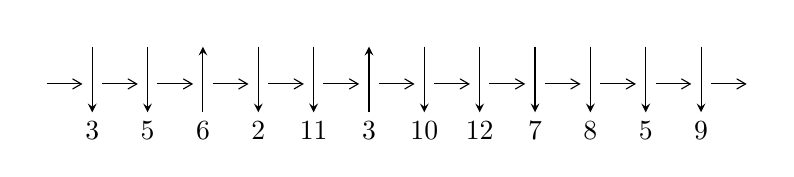
\begin{tikzpicture}[x=20pt, y=17pt]
	% nodes
	\node (C0) at (0, 0) {};
	\node (C1) at (1, 0) {};
	\node (C1U) at (1, +1) {};
	\node (C1D) at (1, -1) {3};

	\node (C2) at (2, 0) {};
	\node (C2U) at (2, +1) {};
	\node (C2D) at (2, -1) {5};

	\node (C3) at (3, 0) {};
	\node (C3U) at (3, +1) {};
	\node (C3D) at (3, -1) {6};

	\node (C4) at (4, 0) {};
	\node (C4U) at (4, +1) {};
	\node (C4D) at (4, -1) {2};

	\node (C5) at (5, 0) {};
	\node (C5U) at (5, +1) {};
	\node (C5D) at (5, -1) {11};

	\node (C6) at (6, 0) {};
	\node (C6U) at (6, +1) {};
	\node (C6D) at (6, -1) {3};

	\node (C7) at (7, 0) {};
	\node (C7U) at (7, +1) {};
	\node (C7D) at (7, -1) {10};

	\node (C8) at (8, 0) {};
	\node (C8U) at (8, +1) {};
	\node (C8D) at (8, -1) {12};

	\node (C9) at (9, 0) {};
	\node (C9U) at (9, +1) {};
	\node (C9D) at (9, -1) {7};

	\node (C10) at (10, 0) {};
	\node (C10U) at (10, +1) {};
	\node (C10D) at (10, -1) {8};

	\node (C11) at (11, 0) {};
	\node (C11U) at (11, +1) {};
	\node (C11D) at (11, -1) {5};

	\node (C12) at (12, 0) {};
	\node (C12U) at (12, +1) {};
	\node (C12D) at (12, -1) {9};
	\node (C13) at (13, 0) {};

	% arrows
	\draw[->,>={angle 60}]
	(C0) edge (C1) (C1) edge (C2) (C2) edge (C3) (C3) edge (C4) (C4) edge (C5) (C5) edge (C6) (C6) edge (C7) (C7) edge (C8) (C8) edge (C9) (C9) edge (C10) (C10) edge (C11) (C11) edge (C12) (C12) edge (C13) ;	\draw[->,>=stealth]
	(C1U) edge (C1D) (C2U) edge (C2D) (C3D) edge (C3U) (C4U) edge (C4D) (C5U) edge (C5D) (C6D) edge (C6U) (C7U) edge (C7D) (C8U) edge (C8D) (C9U) edge (C9D) (C10U) edge (C10D) (C11U) edge (C11D) (C12U) edge (C12D) ;
	\end{tikzpicture} \\
\hhline{~~} \\& 
\textbf{Solving Sequence} \\ \cline{2-2} 
 &
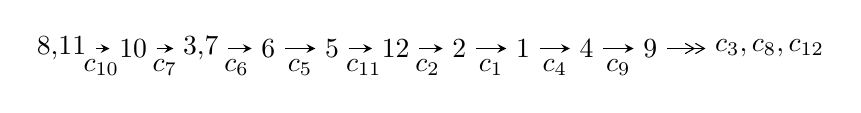
\begin{tikzpicture}[x=23pt, y=7pt]
	% node
	\node (A0) at (-1/8, 0) {8,11};
	\node (A1) at (1, 0) {10};
	\node (A2) at (33/16, 0) {3,7};
	\node (A3) at (25/8, 0) {6};
	\node (A4) at (33/8, 0) {5};
	\node (A5) at (41/8, 0) {12};
	\node (A6) at (49/8, 0) {2};
	\node (A7) at (57/8, 0) {1};
	\node (A8) at (65/8, 0) {4};
	\node (A9) at (73/8, 0) {9};
	\node (C1) at (1/2, -1) {$c_{10}$};
	\node (C2) at (3/2, -1) {$c_{7}$};
	\node (C3) at (21/8, -1) {$c_{6}$};
	\node (C4) at (29/8, -1) {$c_{5}$};
	\node (C5) at (37/8, -1) {$c_{11}$};
	\node (C6) at (45/8, -1) {$c_{2}$};
	\node (C7) at (53/8, -1) {$c_{1}$};
	\node (C8) at (61/8, -1) {$c_{4}$};
	\node (C9) at (69/8, -1) {$c_{9}$};
	\node (A10) at (11, 0) {$c_{3},c_{8},c_{12}$};

	% edge
	\draw[->,>=stealth]	
	(A0) edge (A1) (A1) edge (A2) (A2) edge (A3) (A3) edge (A4) (A4) edge (A5) (A5) edge (A6) (A6) edge (A7) (A7) edge (A8) (A8) edge (A9) ;
	\draw[->>,>={angle 60}]	
	(A9) edge (A10);
\end{tikzpicture} \\ 

\end{tabular} \\

\footnotetext{
The image of knot diagram is generated by the software ``\textbf{Draw programme}" developed by Andrew Bartholomew(\url{http://www.layer8.co.uk/maths/draw/index.htm\#Running-draw}), where we modified some parts for our purpose(\url{https://github.com/CATsTAILs/LinksPainter}).
}\phantom \\ \newline 
\centering \textbf{Ideals for irreducible components\footnotemark of $X_{\text{par}}$} 
 
\begin{align*}
I^u_{1}&=\langle 
-2.24021\times10^{18} u^{33}+1.24343\times10^{19} u^{32}+\cdots+3.99716\times10^{18} b+8.38466\times10^{18},\\
\phantom{I^u_{1}}&\phantom{= \langle  }6.30553\times10^{18} u^{33}-4.12415\times10^{19} u^{32}+\cdots+3.99716\times10^{18} a-2.46809\times10^{18},\;u^{34}-7 u^{33}+\cdots+2 u+1\rangle \\
I^u_{2}&=\langle 
u^7-2 u^6-2 u^5+4 u^4+2 u^3- u^2+b- u-3,\;2 u^7-2 u^6-5 u^5+4 u^4+3 u^3+a+u-3,\\
\phantom{I^u_{2}}&\phantom{= \langle  }u^8- u^7-3 u^6+2 u^5+3 u^4-2 u-1\rangle \\
I^u_{3}&=\langle 
a^4+6 a^3+9 a^2+b+8 a+3,\;a^5+6 a^4+9 a^3+8 a^2+4 a+1,\;u+1\rangle \\
\\
\end{align*}
\raggedright * 3 irreducible components of $\dim_{\mathbb{C}}=0$, with total 47 representations.\\
\footnotetext{All coefficients of polynomials are rational numbers. But the coefficients are sometimes approximated in decimal forms when there is not enough margin.}
\newpage
\renewcommand{\arraystretch}{1}
\centering \section*{I. $I^u_{1}= \langle -2.24\times10^{18} u^{33}+1.24\times10^{19} u^{32}+\cdots+4.00\times10^{18} b+8.38\times10^{18},\;6.31\times10^{18} u^{33}-4.12\times10^{19} u^{32}+\cdots+4.00\times10^{18} a-2.47\times10^{18},\;u^{34}-7 u^{33}+\cdots+2 u+1 \rangle$}
\flushleft \textbf{(i) Arc colorings}\\
\begin{tabular}{m{7pt} m{180pt} m{7pt} m{180pt} }
\flushright $a_{8}=$&$\begin{pmatrix}0\\u\end{pmatrix}$ \\
\flushright $a_{11}=$&$\begin{pmatrix}1\\0\end{pmatrix}$ \\
\flushright $a_{10}=$&$\begin{pmatrix}1\\- u^2\end{pmatrix}$ \\
\flushright $a_{3}=$&$\begin{pmatrix}-1.57750 u^{33}+10.3177 u^{32}+\cdots+58.2632 u+0.617461\\0.560449 u^{33}-3.11078 u^{32}+\cdots-2.59876 u-2.09765\end{pmatrix}$ \\
\flushright $a_{7}=$&$\begin{pmatrix}u\\- u^3+u\end{pmatrix}$ \\
\flushright $a_{6}=$&$\begin{pmatrix}-0.482803 u^{33}+3.08639 u^{32}+\cdots+19.9484 u+6.63525\\0.416532 u^{33}-2.68773 u^{32}+\cdots-10.0892 u-0.640452\end{pmatrix}$ \\
\flushright $a_{5}=$&$\begin{pmatrix}-0.0662706 u^{33}+0.398662 u^{32}+\cdots+9.85920 u+5.99480\\0.416532 u^{33}-2.68773 u^{32}+\cdots-10.0892 u-0.640452\end{pmatrix}$ \\
\flushright $a_{12}=$&$\begin{pmatrix}0.761588 u^{33}-5.20214 u^{32}+\cdots-34.4584 u-1.20581\\-0.232220 u^{33}+1.56116 u^{32}+\cdots+5.13105 u+1.09754\end{pmatrix}$ \\
\flushright $a_{2}=$&$\begin{pmatrix}-1.41061 u^{33}+9.24368 u^{32}+\cdots+55.4109 u-5.35535\\0.349672 u^{33}-1.74827 u^{32}+\cdots+4.90386 u-1.82853\end{pmatrix}$ \\
\flushright $a_{1}=$&$\begin{pmatrix}-0.904188 u^{33}+6.08322 u^{32}+\cdots+37.0080 u+1.94216\\0.467802 u^{33}-2.77338 u^{32}+\cdots-5.68735 u-1.23990\end{pmatrix}$ \\
\flushright $a_{4}=$&$\begin{pmatrix}-1.22385 u^{33}+7.98274 u^{32}+\cdots+53.9857 u-2.86208\\0.480782 u^{33}-2.58022 u^{32}+\cdots+0.0452351 u-1.99768\end{pmatrix}$ \\
\flushright $a_{9}=$&$\begin{pmatrix}- u^2+1\\u^4-2 u^2\end{pmatrix}$\\&\end{tabular}
\flushleft \textbf{(ii) Obstruction class $= -1$}\\~\\
\flushleft \textbf{(iii) Cusp Shapes $= -\frac{2457323729169383761}{1998580887488661448} u^{33}+\frac{19718500600259381097}{1998580887488661448} u^{32}+\cdots+\frac{37446519631365374685}{1998580887488661448} u+\frac{3411256608626139411}{999290443744330724}$}\\~\\
\newpage\renewcommand{\arraystretch}{1}
\flushleft \textbf{(iv) u-Polynomials at the component}\newline \\
\begin{tabular}{m{50pt}|m{274pt}}
Crossings & \hspace{64pt}u-Polynomials at each crossing \\
\hline $$\begin{aligned}c_{1}\end{aligned}$$&$\begin{aligned}
&u^{34}+50 u^{33}+\cdots+7022 u+1
\end{aligned}$\\
\hline $$\begin{aligned}c_{2},c_{4}\end{aligned}$$&$\begin{aligned}
&u^{34}-10 u^{33}+\cdots-94 u+1
\end{aligned}$\\
\hline $$\begin{aligned}c_{3},c_{6}\end{aligned}$$&$\begin{aligned}
&u^{34}+6 u^{33}+\cdots+1408 u+256
\end{aligned}$\\
\hline $$\begin{aligned}c_{5},c_{11}\end{aligned}$$&$\begin{aligned}
&u^{34}-3 u^{33}+\cdots+2 u-1
\end{aligned}$\\
\hline $$\begin{aligned}c_{7},c_{9},c_{10}\end{aligned}$$&$\begin{aligned}
&u^{34}-7 u^{33}+\cdots+2 u+1
\end{aligned}$\\
\hline $$\begin{aligned}c_{8},c_{12}\end{aligned}$$&$\begin{aligned}
&u^{34}+2 u^{33}+\cdots-160 u-32
\end{aligned}$\\
\hline
\end{tabular}\\~\\
\newpage\renewcommand{\arraystretch}{1}
\flushleft \textbf{(v) Riley Polynomials at the component}\newline \\
\begin{tabular}{m{50pt}|m{274pt}}
Crossings & \hspace{64pt}Riley Polynomials at each crossing \\
\hline $$\begin{aligned}c_{1}\end{aligned}$$&$\begin{aligned}
&y^{34}-122 y^{33}+\cdots-49242950 y+1
\end{aligned}$\\
\hline $$\begin{aligned}c_{2},c_{4}\end{aligned}$$&$\begin{aligned}
&y^{34}-50 y^{33}+\cdots-7022 y+1
\end{aligned}$\\
\hline $$\begin{aligned}c_{3},c_{6}\end{aligned}$$&$\begin{aligned}
&y^{34}+54 y^{33}+\cdots-5357568 y+65536
\end{aligned}$\\
\hline $$\begin{aligned}c_{5},c_{11}\end{aligned}$$&$\begin{aligned}
&y^{34}- y^{33}+\cdots-14 y+1
\end{aligned}$\\
\hline $$\begin{aligned}c_{7},c_{9},c_{10}\end{aligned}$$&$\begin{aligned}
&y^{34}-41 y^{33}+\cdots-152 y+1
\end{aligned}$\\
\hline $$\begin{aligned}c_{8},c_{12}\end{aligned}$$&$\begin{aligned}
&y^{34}-36 y^{33}+\cdots-3584 y+1024
\end{aligned}$\\
\hline
\end{tabular}\\~\\
\newpage\flushleft \textbf{(vi) Complex Volumes and Cusp Shapes}
$$\begin{array}{c|c|c}  
\text{Solutions to }I^u_{1}& \I (\text{vol} + \sqrt{-1}CS) & \text{Cusp shape}\\
 \hline 
\begin{aligned}
u &= -0.828237 + 0.495417 I \\
a &= -0.82004 + 1.25784 I \\
b &= -0.297004 - 1.016390 I\end{aligned}
 & -3.57437 + 2.68652 I & -15.9734 - 5.7320 I \\ \hline\begin{aligned}
u &= -0.828237 - 0.495417 I \\
a &= -0.82004 - 1.25784 I \\
b &= -0.297004 + 1.016390 I\end{aligned}
 & -3.57437 - 2.68652 I & -15.9734 + 5.7320 I \\ \hline\begin{aligned}
u &= -1.118840 + 0.182636 I \\
a &= -0.583692 - 0.292922 I \\
b &= -0.076416 - 0.398409 I\end{aligned}
 & -1.23502 + 0.89870 I & -5.08124 + 0.75731 I \\ \hline\begin{aligned}
u &= -1.118840 - 0.182636 I \\
a &= -0.583692 + 0.292922 I \\
b &= -0.076416 + 0.398409 I\end{aligned}
 & -1.23502 - 0.89870 I & -5.08124 - 0.75731 I \\ \hline\begin{aligned}
u &= -1.120600 + 0.202178 I \\
a &= -2.46416 + 1.89535 I \\
b &= \phantom{-}0.325798 - 0.681195 I\end{aligned}
 & -4.37210 - 0.56022 I & -15.7627 + 4.5815 I \\ \hline\begin{aligned}
u &= -1.120600 - 0.202178 I \\
a &= -2.46416 - 1.89535 I \\
b &= \phantom{-}0.325798 + 0.681195 I\end{aligned}
 & -4.37210 + 0.56022 I & -15.7627 - 4.5815 I \\ \hline\begin{aligned}
u &= \phantom{-}0.742537 + 0.037896 I \\
a &= \phantom{-}0.475409 + 1.067840 I \\
b &= -0.412066 - 1.299410 I\end{aligned}
 & -7.07612 + 4.33049 I & -3.74509 - 2.01968 I \\ \hline\begin{aligned}
u &= \phantom{-}0.742537 - 0.037896 I \\
a &= \phantom{-}0.475409 - 1.067840 I \\
b &= -0.412066 + 1.299410 I\end{aligned}
 & -7.07612 - 4.33049 I & -3.74509 + 2.01968 I \\ \hline\begin{aligned}
u &= -0.680778 + 1.106570 I \\
a &= \phantom{-}0.675818 - 0.192256 I \\
b &= \phantom{-}0.34011 + 1.96867 I\end{aligned}
 & -13.7038 + 7.6996 I & -12.45976 - 4.30474 I \\ \hline\begin{aligned}
u &= -0.680778 - 1.106570 I \\
a &= \phantom{-}0.675818 + 0.192256 I \\
b &= \phantom{-}0.34011 - 1.96867 I\end{aligned}
 & -13.7038 - 7.6996 I & -12.45976 + 4.30474 I\\
 \hline 
 \end{array}$$\newpage$$\begin{array}{c|c|c}  
\text{Solutions to }I^u_{1}& \I (\text{vol} + \sqrt{-1}CS) & \text{Cusp shape}\\
 \hline 
\begin{aligned}
u &= -0.658915 + 1.120700 I \\
a &= -0.791484 + 0.062467 I \\
b &= -0.06244 - 1.83419 I\end{aligned}
 & -13.63590 - 0.50051 I & -12.57609 + 0. I\phantom{ +0.000000I} \\ \hline\begin{aligned}
u &= -0.658915 - 1.120700 I \\
a &= -0.791484 - 0.062467 I \\
b &= -0.06244 + 1.83419 I\end{aligned}
 & -13.63590 + 0.50051 I & -12.57609 + 0. I\phantom{ +0.000000I} \\ \hline\begin{aligned}
u &= -0.191366 + 0.643732 I \\
a &= \phantom{-}0.392780 + 0.788789 I \\
b &= \phantom{-}0.215796 + 0.185230 I\end{aligned}
 & \phantom{-}1.50616 + 2.15286 I & -1.89528 - 3.55598 I \\ \hline\begin{aligned}
u &= -0.191366 - 0.643732 I \\
a &= \phantom{-}0.392780 - 0.788789 I \\
b &= \phantom{-}0.215796 - 0.185230 I\end{aligned}
 & \phantom{-}1.50616 - 2.15286 I & -1.89528 + 3.55598 I \\ \hline\begin{aligned}
u &= -0.605994 + 0.208022 I \\
a &= -0.17110 + 2.29061 I \\
b &= -0.87873 + 2.06096 I\end{aligned}
 & -2.48043 + 0.15884 I & -35.3818 - 0.1674 I \\ \hline\begin{aligned}
u &= -0.605994 - 0.208022 I \\
a &= -0.17110 - 2.29061 I \\
b &= -0.87873 - 2.06096 I\end{aligned}
 & -2.48043 - 0.15884 I & -35.3818 + 0.1674 I \\ \hline\begin{aligned}
u &= \phantom{-}1.44687\phantom{ +0.000000I} \\
a &= \phantom{-}0.544436\phantom{ +0.000000I} \\
b &= -0.999548\phantom{ +0.000000I}\end{aligned}
 & -7.19178\phantom{ +0.000000I} & -11.0680\phantom{ +0.000000I} \\ \hline\begin{aligned}
u &= \phantom{-}1.42160 + 0.31037 I \\
a &= \phantom{-}0.011571 - 0.200035 I \\
b &= \phantom{-}0.460927 + 0.211334 I\end{aligned}
 & -3.73420 - 5.65524 I & -8.00000 + 0. I\phantom{ +0.000000I} \\ \hline\begin{aligned}
u &= \phantom{-}1.42160 - 0.31037 I \\
a &= \phantom{-}0.011571 + 0.200035 I \\
b &= \phantom{-}0.460927 - 0.211334 I\end{aligned}
 & -3.73420 + 5.65524 I & -8.00000 + 0. I\phantom{ +0.000000I} \\ \hline\begin{aligned}
u &= -0.489955\phantom{ +0.000000I} \\
a &= -0.772996\phantom{ +0.000000I} \\
b &= -0.364452\phantom{ +0.000000I}\end{aligned}
 & -0.859418\phantom{ +0.000000I} & -11.8170\phantom{ +0.000000I}\\
 \hline 
 \end{array}$$\newpage$$\begin{array}{c|c|c}  
\text{Solutions to }I^u_{1}& \I (\text{vol} + \sqrt{-1}CS) & \text{Cusp shape}\\
 \hline 
\begin{aligned}
u &= \phantom{-}1.67742 + 0.07121 I \\
a &= -0.18227 + 1.86528 I \\
b &= \phantom{-}1.07725 - 2.72182 I\end{aligned}
 & -10.90540 - 1.31562 I & \phantom{-0.000000 } 0 \\ \hline\begin{aligned}
u &= \phantom{-}1.67742 - 0.07121 I \\
a &= -0.18227 - 1.86528 I \\
b &= \phantom{-}1.07725 + 2.72182 I\end{aligned}
 & -10.90540 + 1.31562 I & \phantom{-0.000000 } 0 \\ \hline\begin{aligned}
u &= -1.71439 + 0.00920 I \\
a &= \phantom{-}0.20683 - 1.69911 I \\
b &= -0.11557 + 1.98219 I\end{aligned}
 & -16.1286 - 4.0950 I & \phantom{-0.000000 } 0 \\ \hline\begin{aligned}
u &= -1.71439 - 0.00920 I \\
a &= \phantom{-}0.20683 + 1.69911 I \\
b &= -0.11557 - 1.98219 I\end{aligned}
 & -16.1286 + 4.0950 I & \phantom{-0.000000 } 0 \\ \hline\begin{aligned}
u &= \phantom{-}1.67967 + 0.41006 I \\
a &= \phantom{-}0.59407 + 1.55358 I \\
b &= \phantom{-}0.76478 - 2.07350 I\end{aligned}
 & \phantom{-}18.1726 - 13.4286 I & \phantom{-0.000000 } 0 \\ \hline\begin{aligned}
u &= \phantom{-}1.67967 - 0.41006 I \\
a &= \phantom{-}0.59407 - 1.55358 I \\
b &= \phantom{-}0.76478 + 2.07350 I\end{aligned}
 & \phantom{-}18.1726 + 13.4286 I & \phantom{-0.000000 } 0 \\ \hline\begin{aligned}
u &= \phantom{-}1.67836 + 0.42976 I \\
a &= -0.707434 - 1.159530 I \\
b &= -0.51034 + 1.64958 I\end{aligned}
 & \phantom{-}18.3538 - 5.3451 I & \phantom{-0.000000 } 0 \\ \hline\begin{aligned}
u &= \phantom{-}1.67836 - 0.42976 I \\
a &= -0.707434 + 1.159530 I \\
b &= -0.51034 - 1.64958 I\end{aligned}
 & \phantom{-}18.3538 + 5.3451 I & \phantom{-0.000000 } 0 \\ \hline\begin{aligned}
u &= \phantom{-}1.73009 + 0.14735 I \\
a &= -0.17568 - 1.56407 I \\
b &= -0.48186 + 1.53845 I\end{aligned}
 & -12.71500 - 5.35446 I & \phantom{-0.000000 } 0 \\ \hline\begin{aligned}
u &= \phantom{-}1.73009 - 0.14735 I \\
a &= -0.17568 + 1.56407 I \\
b &= -0.48186 - 1.53845 I\end{aligned}
 & -12.71500 + 5.35446 I & \phantom{-0.000000 } 0\\
 \hline 
 \end{array}$$\newpage$$\begin{array}{c|c|c}  
\text{Solutions to }I^u_{1}& \I (\text{vol} + \sqrt{-1}CS) & \text{Cusp shape}\\
 \hline 
\begin{aligned}
u &= \phantom{-}1.77751\phantom{ +0.000000I} \\
a &= -0.420567\phantom{ +0.000000I} \\
b &= -0.892648\phantom{ +0.000000I}\end{aligned}
 & -15.4063\phantom{ +0.000000I} & \phantom{-0.000000 } 0 \\ \hline\begin{aligned}
u &= \phantom{-}0.178439 + 0.031286 I \\
a &= -1.55747 - 3.87733 I \\
b &= \phantom{-}0.336239 + 0.914967 I\end{aligned}
 & -0.57544 + 1.50411 I & -4.52476 - 4.55824 I \\ \hline\begin{aligned}
u &= \phantom{-}0.178439 - 0.031286 I \\
a &= -1.55747 + 3.87733 I \\
b &= \phantom{-}0.336239 - 0.914967 I\end{aligned}
 & -0.57544 - 1.50411 I & -4.52476 + 4.55824 I \\ \hline\begin{aligned}
u &= -0.112437\phantom{ +0.000000I} \\
a &= -6.15718\phantom{ +0.000000I} \\
b &= -1.11629\phantom{ +0.000000I}\end{aligned}
 & -2.28474\phantom{ +0.000000I} & \phantom{-}0.324850\phantom{ +0.000000I}\\
 \hline 
 \end{array}$$\newpage\newpage\renewcommand{\arraystretch}{1}
\centering \section*{II. $I^u_{2}= \langle u^7-2 u^6-2 u^5+4 u^4+2 u^3- u^2+b- u-3,\;2 u^7-2 u^6-5 u^5+4 u^4+3 u^3+a+u-3,\;u^8- u^7-3 u^6+2 u^5+3 u^4-2 u-1 \rangle$}
\flushleft \textbf{(i) Arc colorings}\\
\begin{tabular}{m{7pt} m{180pt} m{7pt} m{180pt} }
\flushright $a_{8}=$&$\begin{pmatrix}0\\u\end{pmatrix}$ \\
\flushright $a_{11}=$&$\begin{pmatrix}1\\0\end{pmatrix}$ \\
\flushright $a_{10}=$&$\begin{pmatrix}1\\- u^2\end{pmatrix}$ \\
\flushright $a_{3}=$&$\begin{pmatrix}-2 u^7+2 u^6+5 u^5-4 u^4-3 u^3- u+3\\- u^7+2 u^6+2 u^5-4 u^4-2 u^3+u^2+u+3\end{pmatrix}$ \\
\flushright $a_{7}=$&$\begin{pmatrix}u\\- u^3+u\end{pmatrix}$ \\
\flushright $a_{6}=$&$\begin{pmatrix}u\\- u^3+u\end{pmatrix}$ \\
\flushright $a_{5}=$&$\begin{pmatrix}- u^3+2 u\\- u^3+u\end{pmatrix}$ \\
\flushright $a_{12}=$&$\begin{pmatrix}u^6-3 u^4+2 u^2+1\\u^6-2 u^4+u^2\end{pmatrix}$ \\
\flushright $a_{2}=$&$\begin{pmatrix}-2 u^7+2 u^6+5 u^5-4 u^4-2 u^3-3 u+3\\- u^7+2 u^6+2 u^5-4 u^4- u^3+u^2+3\end{pmatrix}$ \\
\flushright $a_{1}=$&$\begin{pmatrix}u^3-2 u\\u^3- u\end{pmatrix}$ \\
\flushright $a_{4}=$&$\begin{pmatrix}-2 u^7+2 u^6+5 u^5-4 u^4-3 u^3- u+3\\- u^7+2 u^6+2 u^5-4 u^4-2 u^3+u^2+u+3\end{pmatrix}$ \\
\flushright $a_{9}=$&$\begin{pmatrix}- u^2+1\\u^4-2 u^2\end{pmatrix}$\\&\end{tabular}
\flushleft \textbf{(ii) Obstruction class $= 1$}\\~\\
\flushleft \textbf{(iii) Cusp Shapes $= 21 u^7-38 u^6-48 u^5+85 u^4+39 u^3-27 u^2-5 u-70$}\\~\\
\newpage\renewcommand{\arraystretch}{1}
\flushleft \textbf{(iv) u-Polynomials at the component}\newline \\
\begin{tabular}{m{50pt}|m{274pt}}
Crossings & \hspace{64pt}u-Polynomials at each crossing \\
\hline $$\begin{aligned}c_{1},c_{2}\end{aligned}$$&$\begin{aligned}
&(u-1)^8
\end{aligned}$\\
\hline $$\begin{aligned}c_{3},c_{6}\end{aligned}$$&$\begin{aligned}
&u^8
\end{aligned}$\\
\hline $$\begin{aligned}c_{4}\end{aligned}$$&$\begin{aligned}
&(u+1)^8
\end{aligned}$\\
\hline $$\begin{aligned}c_{5}\end{aligned}$$&$\begin{aligned}
&u^8-3 u^7+7 u^6-10 u^5+11 u^4-10 u^3+6 u^2-4 u+1
\end{aligned}$\\
\hline $$\begin{aligned}c_{7}\end{aligned}$$&$\begin{aligned}
&u^8+u^7-3 u^6-2 u^5+3 u^4+2 u-1
\end{aligned}$\\
\hline $$\begin{aligned}c_{8}\end{aligned}$$&$\begin{aligned}
&u^8- u^7- u^6+2 u^5+u^4-2 u^3+2 u-1
\end{aligned}$\\
\hline $$\begin{aligned}c_{9},c_{10}\end{aligned}$$&$\begin{aligned}
&u^8- u^7-3 u^6+2 u^5+3 u^4-2 u-1
\end{aligned}$\\
\hline $$\begin{aligned}c_{11}\end{aligned}$$&$\begin{aligned}
&u^8+3 u^7+7 u^6+10 u^5+11 u^4+10 u^3+6 u^2+4 u+1
\end{aligned}$\\
\hline $$\begin{aligned}c_{12}\end{aligned}$$&$\begin{aligned}
&u^8+u^7- u^6-2 u^5+u^4+2 u^3-2 u-1
\end{aligned}$\\
\hline
\end{tabular}\\~\\
\newpage\renewcommand{\arraystretch}{1}
\flushleft \textbf{(v) Riley Polynomials at the component}\newline \\
\begin{tabular}{m{50pt}|m{274pt}}
Crossings & \hspace{64pt}Riley Polynomials at each crossing \\
\hline $$\begin{aligned}c_{1},c_{2},c_{4}\end{aligned}$$&$\begin{aligned}
&(y-1)^8
\end{aligned}$\\
\hline $$\begin{aligned}c_{3},c_{6}\end{aligned}$$&$\begin{aligned}
&y^8
\end{aligned}$\\
\hline $$\begin{aligned}c_{5},c_{11}\end{aligned}$$&$\begin{aligned}
&y^8+5 y^7+11 y^6+6 y^5-17 y^4-34 y^3-22 y^2-4 y+1
\end{aligned}$\\
\hline $$\begin{aligned}c_{7},c_{9},c_{10}\end{aligned}$$&$\begin{aligned}
&y^8-7 y^7+19 y^6-22 y^5+3 y^4+14 y^3-6 y^2-4 y+1
\end{aligned}$\\
\hline $$\begin{aligned}c_{8},c_{12}\end{aligned}$$&$\begin{aligned}
&y^8-3 y^7+7 y^6-10 y^5+11 y^4-10 y^3+6 y^2-4 y+1
\end{aligned}$\\
\hline
\end{tabular}\\~\\
\newpage\flushleft \textbf{(vi) Complex Volumes and Cusp Shapes}
$$\begin{array}{c|c|c}  
\text{Solutions to }I^u_{2}& \I (\text{vol} + \sqrt{-1}CS) & \text{Cusp shape}\\
 \hline 
\begin{aligned}
u &= -1.180120 + 0.268597 I \\
a &= -1.23903 + 1.07030 I \\
b &= -0.281371 - 1.128550 I\end{aligned}
 & -2.68559 + 1.13123 I & -12.74421 + 0.55338 I \\ \hline\begin{aligned}
u &= -1.180120 - 0.268597 I \\
a &= -1.23903 - 1.07030 I \\
b &= -0.281371 + 1.128550 I\end{aligned}
 & -2.68559 - 1.13123 I & -12.74421 - 0.55338 I \\ \hline\begin{aligned}
u &= -0.108090 + 0.747508 I \\
a &= \phantom{-}0.188536 + 0.513699 I \\
b &= \phantom{-}0.208670 + 0.825203 I\end{aligned}
 & \phantom{-}0.51448 + 2.57849 I & -9.60894 - 4.72239 I \\ \hline\begin{aligned}
u &= -0.108090 - 0.747508 I \\
a &= \phantom{-}0.188536 - 0.513699 I \\
b &= \phantom{-}0.208670 - 0.825203 I\end{aligned}
 & \phantom{-}0.51448 - 2.57849 I & -9.60894 + 4.72239 I \\ \hline\begin{aligned}
u &= \phantom{-}1.37100\phantom{ +0.000000I} \\
a &= -0.942639\phantom{ +0.000000I} \\
b &= \phantom{-}0.829189\phantom{ +0.000000I}\end{aligned}
 & -8.14766\phantom{ +0.000000I} & -20.4520\phantom{ +0.000000I} \\ \hline\begin{aligned}
u &= \phantom{-}1.334530 + 0.318930 I \\
a &= \phantom{-}0.271933 + 0.551071 I \\
b &= \phantom{-}0.284386 - 0.605794 I\end{aligned}
 & -4.02461 - 6.44354 I & -12.4754 + 9.9976 I \\ \hline\begin{aligned}
u &= \phantom{-}1.334530 - 0.318930 I \\
a &= \phantom{-}0.271933 - 0.551071 I \\
b &= \phantom{-}0.284386 + 0.605794 I\end{aligned}
 & -4.02461 + 6.44354 I & -12.4754 - 9.9976 I \\ \hline\begin{aligned}
u &= -0.463640\phantom{ +0.000000I} \\
a &= \phantom{-}3.49976\phantom{ +0.000000I} \\
b &= \phantom{-}2.74744\phantom{ +0.000000I}\end{aligned}
 & -2.48997\phantom{ +0.000000I} & -72.8910\phantom{ +0.000000I}\\
 \hline 
 \end{array}$$\newpage\newpage\renewcommand{\arraystretch}{1}
\centering \section*{III. $I^u_{3}= \langle a^4+6 a^3+9 a^2+b+8 a+3,\;a^5+6 a^4+9 a^3+8 a^2+4 a+1,\;u+1 \rangle$}
\flushleft \textbf{(i) Arc colorings}\\
\begin{tabular}{m{7pt} m{180pt} m{7pt} m{180pt} }
\flushright $a_{8}=$&$\begin{pmatrix}0\\-1\end{pmatrix}$ \\
\flushright $a_{11}=$&$\begin{pmatrix}1\\0\end{pmatrix}$ \\
\flushright $a_{10}=$&$\begin{pmatrix}1\\-1\end{pmatrix}$ \\
\flushright $a_{3}=$&$\begin{pmatrix}a\\- a^4-6 a^3-9 a^2-8 a-3\end{pmatrix}$ \\
\flushright $a_{7}=$&$\begin{pmatrix}-1\\0\end{pmatrix}$ \\
\flushright $a_{6}=$&$\begin{pmatrix}- a-2\\-2 a^4-11 a^3-12 a^2-7 a-1\end{pmatrix}$ \\
\flushright $a_{5}=$&$\begin{pmatrix}-2 a^4-11 a^3-12 a^2-8 a-3\\-2 a^4-11 a^3-12 a^2-7 a-1\end{pmatrix}$ \\
\flushright $a_{12}=$&$\begin{pmatrix}0\\-3 a^4-16 a^3-15 a^2-7 a-1\end{pmatrix}$ \\
\flushright $a_{2}=$&$\begin{pmatrix}a^3+5 a^2+5 a+2\\-2 a^4-12 a^3-17 a^2-11 a-3\end{pmatrix}$ \\
\flushright $a_{1}=$&$\begin{pmatrix}0\\-3 a^4-16 a^3-15 a^2-7 a-1\end{pmatrix}$ \\
\flushright $a_{4}=$&$\begin{pmatrix}-2 a^4-12 a^3-18 a^2-14 a-5\\a^3+5 a^2+3 a+1\end{pmatrix}$ \\
\flushright $a_{9}=$&$\begin{pmatrix}0\\-1\end{pmatrix}$\\&\end{tabular}
\flushleft \textbf{(ii) Obstruction class $= 1$}\\~\\
\flushleft \textbf{(iii) Cusp Shapes $= -7 a^4-32 a^3-8 a^2-12$}\\~\\
\newpage\renewcommand{\arraystretch}{1}
\flushleft \textbf{(iv) u-Polynomials at the component}\newline \\
\begin{tabular}{m{50pt}|m{274pt}}
Crossings & \hspace{64pt}u-Polynomials at each crossing \\
\hline $$\begin{aligned}c_{1}\end{aligned}$$&$\begin{aligned}
&u^5-5 u^4+8 u^3-3 u^2- u-1
\end{aligned}$\\
\hline $$\begin{aligned}c_{2}\end{aligned}$$&$\begin{aligned}
&u^5+u^4-2 u^3- u^2+u-1
\end{aligned}$\\
\hline $$\begin{aligned}c_{3}\end{aligned}$$&$\begin{aligned}
&u^5- u^4+2 u^3- u^2+u-1
\end{aligned}$\\
\hline $$\begin{aligned}c_{4}\end{aligned}$$&$\begin{aligned}
&u^5- u^4-2 u^3+u^2+u+1
\end{aligned}$\\
\hline $$\begin{aligned}c_{5}\end{aligned}$$&$\begin{aligned}
&u^5+3 u^4+4 u^3+u^2- u-1
\end{aligned}$\\
\hline $$\begin{aligned}c_{6}\end{aligned}$$&$\begin{aligned}
&u^5+u^4+2 u^3+u^2+u+1
\end{aligned}$\\
\hline $$\begin{aligned}c_{7}\end{aligned}$$&$\begin{aligned}
&(u-1)^5
\end{aligned}$\\
\hline $$\begin{aligned}c_{8},c_{12}\end{aligned}$$&$\begin{aligned}
&u^5
\end{aligned}$\\
\hline $$\begin{aligned}c_{9},c_{10}\end{aligned}$$&$\begin{aligned}
&(u+1)^5
\end{aligned}$\\
\hline $$\begin{aligned}c_{11}\end{aligned}$$&$\begin{aligned}
&u^5-3 u^4+4 u^3- u^2- u+1
\end{aligned}$\\
\hline
\end{tabular}\\~\\
\newpage\renewcommand{\arraystretch}{1}
\flushleft \textbf{(v) Riley Polynomials at the component}\newline \\
\begin{tabular}{m{50pt}|m{274pt}}
Crossings & \hspace{64pt}Riley Polynomials at each crossing \\
\hline $$\begin{aligned}c_{1}\end{aligned}$$&$\begin{aligned}
&y^5-9 y^4+32 y^3-35 y^2-5 y-1
\end{aligned}$\\
\hline $$\begin{aligned}c_{2},c_{4}\end{aligned}$$&$\begin{aligned}
&y^5-5 y^4+8 y^3-3 y^2- y-1
\end{aligned}$\\
\hline $$\begin{aligned}c_{3},c_{6}\end{aligned}$$&$\begin{aligned}
&y^5+3 y^4+4 y^3+y^2- y-1
\end{aligned}$\\
\hline $$\begin{aligned}c_{5},c_{11}\end{aligned}$$&$\begin{aligned}
&y^5- y^4+8 y^3-3 y^2+3 y-1
\end{aligned}$\\
\hline $$\begin{aligned}c_{7},c_{9},c_{10}\end{aligned}$$&$\begin{aligned}
&(y-1)^5
\end{aligned}$\\
\hline $$\begin{aligned}c_{8},c_{12}\end{aligned}$$&$\begin{aligned}
&y^5
\end{aligned}$\\
\hline
\end{tabular}\\~\\
\newpage\flushleft \textbf{(vi) Complex Volumes and Cusp Shapes}
$$\begin{array}{c|c|c}  
\text{Solutions to }I^u_{3}& \I (\text{vol} + \sqrt{-1}CS) & \text{Cusp shape}\\
 \hline 
\begin{aligned}
u &= -1.00000\phantom{ +0.000000I} \\
a &= -0.313425 + 0.691081 I \\
b &= \phantom{-}0.455697 - 1.200150 I\end{aligned}
 & -7.51750 - 4.40083 I & -22.0438 + 5.2094 I \\ \hline\begin{aligned}
u &= -1.00000\phantom{ +0.000000I} \\
a &= -0.313425 - 0.691081 I \\
b &= \phantom{-}0.455697 + 1.200150 I\end{aligned}
 & -7.51750 + 4.40083 I & -22.0438 - 5.2094 I \\ \hline\begin{aligned}
u &= -1.00000\phantom{ +0.000000I} \\
a &= -0.542256 + 0.333011 I \\
b &= -0.339110 - 0.822375 I\end{aligned}
 & -1.97403 + 1.53058 I & -13.4575 - 4.4032 I \\ \hline\begin{aligned}
u &= -1.00000\phantom{ +0.000000I} \\
a &= -0.542256 - 0.333011 I \\
b &= -0.339110 + 0.822375 I\end{aligned}
 & -1.97403 - 1.53058 I & -13.4575 + 4.4032 I \\ \hline\begin{aligned}
u &= -1.00000\phantom{ +0.000000I} \\
a &= -4.28864\phantom{ +0.000000I} \\
b &= \phantom{-}0.766826\phantom{ +0.000000I}\end{aligned}
 & -4.04602\phantom{ +0.000000I} & -2.99730\phantom{ +0.000000I}\\
 \hline 
 \end{array}$$\newpage
\newpage\renewcommand{\arraystretch}{1}
\centering \section*{ IV. u-Polynomials}
\begin{tabular}{m{50pt}|m{274pt}}
Crossings & \hspace{64pt}u-Polynomials at each crossing \\
\hline $$\begin{aligned}c_{1}\end{aligned}$$&$\begin{aligned}
&((u-1)^8)(u^5-5 u^4+\cdots- u-1)(u^{34}+50 u^{33}+\cdots+7022 u+1)
\end{aligned}$\\
\hline $$\begin{aligned}c_{2}\end{aligned}$$&$\begin{aligned}
&((u-1)^8)(u^5+u^4+\cdots+u-1)(u^{34}-10 u^{33}+\cdots-94 u+1)
\end{aligned}$\\
\hline $$\begin{aligned}c_{3}\end{aligned}$$&$\begin{aligned}
&u^8(u^5- u^4+\cdots+u-1)(u^{34}+6 u^{33}+\cdots+1408 u+256)
\end{aligned}$\\
\hline $$\begin{aligned}c_{4}\end{aligned}$$&$\begin{aligned}
&((u+1)^8)(u^5- u^4+\cdots+u+1)(u^{34}-10 u^{33}+\cdots-94 u+1)
\end{aligned}$\\
\hline $$\begin{aligned}c_{5}\end{aligned}$$&$\begin{aligned}
&(u^5+3 u^4+4 u^3+u^2- u-1)\\
&\cdot(u^8-3 u^7+7 u^6-10 u^5+11 u^4-10 u^3+6 u^2-4 u+1)\\
&\cdot(u^{34}-3 u^{33}+\cdots+2 u-1)
\end{aligned}$\\
\hline $$\begin{aligned}c_{6}\end{aligned}$$&$\begin{aligned}
&u^8(u^5+u^4+\cdots+u+1)(u^{34}+6 u^{33}+\cdots+1408 u+256)
\end{aligned}$\\
\hline $$\begin{aligned}c_{7}\end{aligned}$$&$\begin{aligned}
&((u-1)^5)(u^8+u^7+\cdots+2 u-1)(u^{34}-7 u^{33}+\cdots+2 u+1)
\end{aligned}$\\
\hline $$\begin{aligned}c_{8}\end{aligned}$$&$\begin{aligned}
&u^5(u^8- u^7+\cdots+2 u-1)(u^{34}+2 u^{33}+\cdots-160 u-32)
\end{aligned}$\\
\hline $$\begin{aligned}c_{9},c_{10}\end{aligned}$$&$\begin{aligned}
&((u+1)^5)(u^8- u^7+\cdots-2 u-1)(u^{34}-7 u^{33}+\cdots+2 u+1)
\end{aligned}$\\
\hline $$\begin{aligned}c_{11}\end{aligned}$$&$\begin{aligned}
&(u^5-3 u^4+4 u^3- u^2- u+1)\\
&\cdot(u^8+3 u^7+7 u^6+10 u^5+11 u^4+10 u^3+6 u^2+4 u+1)\\
&\cdot(u^{34}-3 u^{33}+\cdots+2 u-1)
\end{aligned}$\\
\hline $$\begin{aligned}c_{12}\end{aligned}$$&$\begin{aligned}
&u^5(u^8+u^7+\cdots-2 u-1)(u^{34}+2 u^{33}+\cdots-160 u-32)
\end{aligned}$\\
\hline
\end{tabular}\newpage\renewcommand{\arraystretch}{1}
\centering \section*{ V. Riley Polynomials}
\begin{tabular}{m{50pt}|m{274pt}}
Crossings & \hspace{64pt}Riley Polynomials at each crossing \\
\hline $$\begin{aligned}c_{1}\end{aligned}$$&$\begin{aligned}
&(y-1)^8(y^5-9 y^4+32 y^3-35 y^2-5 y-1)\\
&\cdot(y^{34}-122 y^{33}+\cdots-49242950 y+1)
\end{aligned}$\\
\hline $$\begin{aligned}c_{2},c_{4}\end{aligned}$$&$\begin{aligned}
&((y-1)^8)(y^5-5 y^4+\cdots- y-1)(y^{34}-50 y^{33}+\cdots-7022 y+1)
\end{aligned}$\\
\hline $$\begin{aligned}c_{3},c_{6}\end{aligned}$$&$\begin{aligned}
&y^8(y^5+3 y^4+\cdots- y-1)(y^{34}+54 y^{33}+\cdots-5357568 y+65536)
\end{aligned}$\\
\hline $$\begin{aligned}c_{5},c_{11}\end{aligned}$$&$\begin{aligned}
&(y^5- y^4+8 y^3-3 y^2+3 y-1)\\
&\cdot(y^8+5 y^7+11 y^6+6 y^5-17 y^4-34 y^3-22 y^2-4 y+1)\\
&\cdot(y^{34}- y^{33}+\cdots-14 y+1)
\end{aligned}$\\
\hline $$\begin{aligned}c_{7},c_{9},c_{10}\end{aligned}$$&$\begin{aligned}
&(y-1)^5(y^8-7 y^7+19 y^6-22 y^5+3 y^4+14 y^3-6 y^2-4 y+1)\\
&\cdot(y^{34}-41 y^{33}+\cdots-152 y+1)
\end{aligned}$\\
\hline $$\begin{aligned}c_{8},c_{12}\end{aligned}$$&$\begin{aligned}
&y^5(y^8-3 y^7+7 y^6-10 y^5+11 y^4-10 y^3+6 y^2-4 y+1)\\
&\cdot(y^{34}-36 y^{33}+\cdots-3584 y+1024)
\end{aligned}$\\
\hline
\end{tabular}
\vskip 2pc
\end{document}